\documentclass[10pt,conference]{article}
% GHI CHU: dung class 'article' tam thoi de bien dich duoc ngay khong can
% file .cls rieng. Truoc khi nop that, THAY documentclass nay bang class
% chuan cua venue (vd IEEEtran cho IEEE CoG/ToG, hoac class cua ICAPS/AAAI
% workshop) -- moi venue co yeu cau khac nhau ve margin/font/column.

\usepackage[utf8]{inputenc}
\usepackage[T1]{fontenc}   % T1 du dung cho ten tac gia co dau (vd Swiechowski,
                            % Slezak). KHONG dung T5 -- goi nay khong co san
                            % trong nhieu ban TeXLive toi gian (da xac nhan
                            % gay loi "Encoding scheme T5 unknown" lap lai
                            % hang chuc lan, tuy pdflatex van xuat PDF trong
                            % nonstopmode do bo qua loi).
                            %
                            % LUU Y: goi lmodern (font hien dai, ToUnicode
                            % chinh xac hon) KHONG co san trong may sandbox
                            % dung de soan file nay (khong tai duoc goi TeX
                            % qua mang). Voi Computer Modern mac dinh + T1,
                            % cac ky tu co dau kieu Ba Lan (\'S, \k{e} trong
                            % ten tac gia Swiechowski/Slezak) HIEN THI DUNG
                            % tren PDF (da kiem chung bang anh render), nhung
                            % pdftotext/copy-paste co the trich sai dau (gioi
                            % han da biet cua CM font, khong phai loi bien
                            % dich). Neu co TeXLive day du (vd Overleaf),
                            % NEN them \usepackage{lmodern} de sua triet de.
\usepackage{amsmath,amssymb}
\usepackage{graphicx}
\usepackage{booktabs}
\usepackage{hyperref}
\usepackage[numbers]{natbib}
\usepackage{xcolor}

\newcommand{\todo}[1]{\textcolor{red}{\textbf{[TODO: #1]}}}

\title{Quantifying and Improving Human-Likeness in AI-Generated CFOP
Solutions for Rubik's Cube: A Trigger-Biased Search Approach}

% GHI CHU: doi ten tac gia/don vi truoc khi nop. Xoa comment neu venue
% yeu cau double-blind (thuong phai an danh ban thao khi submit).
\author{
  Pham Dang Khue \\
  Faculty of Information Technology, Electric Power University\\
  pdkhue2004@gmail.com
}

\date{}

\begin{document}
\maketitle

% ============================================================
\begin{abstract}
Existing computational approaches to solving the Rubik's Cube --
including pattern-database search \citep{korf1997}, group-theoretic
optimal solvers \citep{rokicki2014,kociemba}, and reinforcement
learning \citep{mcaleer2018} -- optimize almost exclusively for move
count, producing solutions that are correct but largely
uninterpretable to human learners. In contrast, the human-designed
CFOP method (Cross, F2L, OLL, PLL) trades move-count optimality for
learnability, structured around a finite set of memorable
move-sequence patterns (``algorithms''). We formalize the notion of
\emph{human-likeness} of a cube-solving plan in the vocabulary of
human-aware AI planning \citep{kulkarni2016,chakraborti2019},
propose a composite \emph{Human-Likeness Index} (HLI) built from
three measurable components (stage segmentability, named-algorithm
pattern-conformity, and finger-trick trigger-overlap), and introduce
\emph{Trigger-Biased A* Search}, a heuristic-search modification that
explicitly rewards search branches overlapping with a corpus of
human finger-tricks. Pilot experiments (N=60 random-state scrambles
for the baseline comparison, robustness-checked on N=100 random-move
scrambles, N=60 for the Pareto sweep) show that biasing the F2L
search heuristic increases
trigger-overlap from a baseline of 9.0\% to 25.5\% at $\lambda=1.0$
(Wilcoxon $p=8.3\times10^{-8}$), at a move-count cost of only 7.4\%
(Wilcoxon $p=0.0014$), revealing a favorable, though non-linear (in
compute time), Pareto trade-off. A blinded, BotPrize-style
\citep{hingston2009} human-judge study (24 stimuli, 28 raters)
confirms HLI's construct validity (Spearman $\rho=0.487$,
$p=0.016$ against mean human-likeness ratings) and shows that
Trigger-Biased Search moves AI-generated solves from
statistically-distinguishable-from-human ($p=0.005$) to
statistically-indistinguishable-from-human ($p=0.109$) in blinded
judgment. This work is, to our knowledge, the first
to apply explicability-style metrics to a large combinatorial search
domain, bridging classical heuristic search AI with human-aware and
believable-agent AI research.
\end{abstract}

% ============================================================
\section{Introduction}
\label{sec:intro}

Solving the Rubik's Cube has long served as a benchmark domain for
heuristic search and combinatorial optimization
\citep{korf1997,rokicki2014}, and more recently for
self-play reinforcement learning \citep{mcaleer2018}. These
approaches share a common objective: minimizing the number of moves
(or maximizing win rate against an adversarial scrambler), with no
regard for whether the resulting solution corresponds to any
recognizable pattern a human could learn, memorize, or explain.

Human speedcubers, in contrast, use structured methods such as CFOP
(Cross, F2L, OLL, PLL), deliberately trading move-count optimality
for \emph{learnability}: each stage reduces to recognizing one of a
bounded number of canonical ``cases,'' each paired with a fixed,
named algorithm. The full CFOP method comprises 57 named OLL cases
and 21 named PLL cases; a widely-used simplified variant
(``2-look OLL/PLL'') solves each stage in two sequential passes using
a much smaller subset of algorithms, at the cost of extra moves. Our
system implements a verified table of all 21 PLL cases
(Section~\ref{sec:hli-conformity}). At the time the experiments
reported in this paper were run, OLL coverage was limited to a
2-look decomposition (2 generator algorithms, Sune/Anti-Sune, rather
than the full 57); this asymmetry is itself informative for
Pattern-conformity measurement (Section~\ref{sec:method}). The
solver has since been extended to a single-look table with all 57
cases functionally verified (each confirmed not to break Cross+F2L
when applied from a solved state, via
\texttt{verify\_and\_build\_table()}); of these, 40 of 57 have been
matched against the standard community numbering (increasing over
successive review passes), with the remaining 17 functionally valid
but not yet matched to a specific community number. For OLL~2 and
OLL~20 specifically: every pure face-turn algorithm (no
slice/wide moves) published by the speedcubing community for these
two cases uses a slice or wide move (M/S/E or r/l/f/u/d/b) --- this
is an \emph{empirical observation} from public sources, \textbf{not}
a formal proof by exhaustive search (no such script exists in this
repository); these two cases therefore still fall back to the
verified 2-look decomposition. This upgrade postdates data
collection and does not alter the results reported in
Section~\ref{sec:results}, which reflect the 2-generator OLL table
described above.

Three related research directions (Section~\ref{sec:related}) currently
do not intersect: computer-optimal Rubik's Cube solvers
(Section~\ref{sec:related-optimal}) disregard interpretability entirely;
human-aware AI planning (Section~\ref{sec:related-explicability}) has
formalized explicability but only for small-scale symbolic
task-planning problems, not for a large-scale combinatorial search
domain such as the Rubik's Cube; and the game-AI community
(Section~\ref{sec:related-believability}) has developed a rigorous
blinded human-judge methodology for measuring human-likeness
(BotPrize) but has never applied it to a combinatorial puzzle-solving
agent. The closest CFOP tutoring system (ALLURE,
Section~\ref{sec:related-allure}) covers only the Cross sub-goal and
reports no comparable blinded human-likeness evaluation. This paper
closes that gap by combining all three threads: a human-likeness
metric formalized in the vocabulary of explicability, a search
mechanism that explicitly optimizes for that metric, and a blinded
human-judge study that validates both.

\paragraph{Contributions.} This paper makes the following contributions:
\begin{enumerate}
  \item A formalization of \emph{human-likeness} for cube-solving
    plans grounded in the human-aware planning notion of
    explicability \citep{kulkarni2016,chakraborti2019}, instantiated
    as a composite \textbf{Human-Likeness Index (HLI)} with three
    measurable, reproducible components (Section~\ref{sec:method}).
  \item \textbf{Trigger-Biased A* Search}: a minimal, backward-compatible
    modification to pattern-database-guided A* search for F2L that
    explicitly optimizes for human finger-trick overlap via a single
    interpretable hyperparameter $\lambda$ (Section~\ref{sec:method}).
  \item An empirical Pareto analysis of the human-likeness /
    move-count / compute-time trade-off induced by $\lambda$
    (Section~\ref{sec:results}).
  \item A blinded, BotPrize-style \citep{hingston2009} human-judge
    study (24 stimuli, 28 raters) that both construct-validates HLI
    against human judgment and shows Trigger-Biased Search closes
    the human-likeness gap to statistical
    indistinguishability from real human solves
    (Section~\ref{sec:exp3}).
\end{enumerate}

% ============================================================
\section{Related Work}
\label{sec:related}

\subsection{Computer-optimal Rubik's Cube solvers}
\label{sec:related-optimal}
Korf's IDA* with additive pattern databases \citep{korf1997} was the
first method to find provably optimal solutions for arbitrary
scrambles. Rokicki et al.\ \citep{rokicki2014} established that every
cube state is solvable within 20 face turns (``God's Number''), via
large-scale coset-based search. Kociemba's two-phase algorithm
\citep{kociemba} trades strict optimality for tractable runtime,
typically returning solutions within 1--4 moves of optimal, and is
the baseline we use in Section~\ref{sec:setup}. McAleer et al.\
\citep{mcaleer2018} showed a reinforcement-learning agent
(DeepCubeA) can learn to solve the cube without built-in human
knowledge, achieving near-optimal solution lengths. None of these
methods produce plans that are segmentable, named, or otherwise
interpretable in terms any human learner would recognize --- they are,
in our terminology, maximally \emph{computer-like}.

\subsection{Human-aware planning and explicability}
\label{sec:related-explicability}
A separate line of work in AI planning studies how autonomous agents
should behave when observed or assisted by humans with an internal,
possibly imperfect mental model of the agent. Kulkarni et
al.\ \citep{kulkarni2016} formalize \emph{explicability} as
minimizing the distance between an agent's actual plan and the plan
the human observer expects, and propose search modifications that
bias planning toward more explicable trajectories --- structurally
analogous to the trigger-biased heuristic we propose in
Section~\ref{sec:method}, but applied here to symbolic task planning
rather than a large combinatorial puzzle domain. Chakraborti et
al.\ \citep{chakraborti2019} survey this landscape (explicability,
legibility, predictability, transparency), which we adopt as the
theoretical vocabulary for this paper. Zhang et al.\ \citep{zhang2017}
propose a way to compute explicability/predictability specifically
for robot task planning by learning a labeling function from
training data, in contrast to the direct, learning-free measurement
approach we use for HLI's components (Section~\ref{sec:method}).

\subsection{Human-likeness / believability of game-playing agents}
\label{sec:related-believability}
Independently, the game-AI community has long studied how to make
autonomous agents \emph{appear} human. The 2K BotPrize competition
\citep{hingston2009} operationalized this as a Turing-test variant in
which human judges rate both human and bot players on a 1--5
human-likeness scale, without being told which is which. In the 2012
edition, two bots --- UT\^{}2 (University of Texas at Austin) and
MirrorBot (Mihai Polceanu) --- were the first to cross the 50\%
threshold for being rated human, in fact scoring higher than the
real human players in that year's contest, demonstrating that an
agent explicitly optimized to appear human can outscore actual
humans on that very measure. A recent survey \citep{humanlike2025} frames
human-like game AI research around two questions --- how to
model/implement human-like behavior, and how to measure its degree
--- which we adopt as the organizing structure for this paper's two
main contributions (Sections~\ref{sec:method}).

\subsection{CFOP-specific tutoring systems}
\label{sec:related-allure}
Closest to our work, the ALLURE system \citep{allure} pairs an
automatic solver (DeepCubeA-based search over subgoals) with an
interactive chatbot tutor to help learners understand explainable
solutions to the White Cross sub-goal of CFOP; a recent pilot study
\citep{vanacore2025} (unpublished manuscript at the time of writing)
analyzes student engagement patterns within ALLURE via behavioral
clustering, reporting that the beginner white-cross strategy
requires substantially more moves than CFOP, which in turn requires
more moves than fully optimized methods --- directly
illustrating the learnability/optimality trade-off central to our
formalization (Section~\ref{sec:formalization}). Our work differs in
(a) scope --- covering all four CFOP stages rather than Cross alone
--- (b) mechanism --- an explicit, tunable search bias
(Section~\ref{sec:method}) rather than post-hoc natural-language
explanation of moves already found by an unconstrained solver ---
and (c) evaluation --- neither ALLURE study reports a blinded
human-likeness judgment comparable to our Experiment~3
(Section~\ref{sec:exp3}).

% ============================================================
\section{Problem Formalization}
\label{sec:formalization}

Let $G$ denote the Rubik's Cube group ($|G| \approx 4.3 \times
10^{19}$), and let a \emph{plan} $\pi = (m_1, \ldots, m_k)$ be a
sequence of face-turn generators solving a given scramble $s \in G$.
Let $M_H$ denote a \emph{human expectation model}: in this paper,
$M_H$ is instantiated concretely as (i) the CFOP stage decomposition
(Cross $\to$ F2L $\to$ OLL $\to$ PLL), (ii) a finite table of named,
canonical algorithms for OLL/PLL (Section~\ref{sec:hli-conformity}),
and (iii) a corpus $T$ of short move n-grams (``finger-tricks'')
commonly executed as single motor units by human solvers
(Section~\ref{sec:hli-trigger}).

Following \citet{kulkarni2016}, we define human-likeness as an
(inverse) distance between $\pi$ and the behavior $M_H$ would
consider natural. We instantiate this distance as a weighted sum of
three normalized, independently-measurable components (rather than a
single learned or hand-tuned distance function), described in
Section~\ref{sec:method}.

% ============================================================
\section{Method}
\label{sec:method}

\subsection{Human-Likeness Index (HLI)}

\paragraph{Segmentability $S(\pi) \in \{0,1\}$.}
Equals 1 iff $\pi$ decomposes into four contiguous, independently
verifiable sub-sequences satisfying the Cross, F2L, OLL, and PLL
postconditions in order, and 0 otherwise (e.g.\ for plans that solve
the cube via an undifferentiated optimal sequence, as computer-like
solvers do by construction).

\paragraph{Pattern-conformity $P(\pi) \in [0,1]$.}
\label{sec:hli-conformity}
Restricted to the OLL and PLL stages (where a finite, named
case-to-algorithm mapping exists in CFOP), $P(\pi)$ is the fraction
of solved stages whose corresponding sub-sequence exactly matches an
entry in a verified table of canonical algorithms (Aa, Ab, \ldots,
Z for PLL; Sune/Anti-Sune generators for 2-look OLL, the table in
effect at data-collection time --- see Section~\ref{sec:intro} for
the subsequent upgrade to a full single-look OLL table, which does
not affect the
figures below) rather than an
unstructured search fallback. All 21/21 PLL cases in the table are
verified automatically on first module import via
\texttt{verify\_and\_build\_table()}
(\texttt{solver/pll\_algorithms.py}); we confirmed this by re-running
the function directly, obtaining exactly 21 verified case names (Aa,
Ab, E, F, Ga, Gb, Gc, Gd, H, Ja, Jb, Na, Nb, Ra, Rb, T, Ua, Ub, V, Y,
Z).

\paragraph{Trigger-overlap $O(\pi) \in [0,1]$.}
\label{sec:hli-trigger}
For the Cross and F2L stages (which lack a canonical case table in
this system, being generated by unconstrained heuristic search), we
measure the fraction of moves covered by a greedy longest-match
segmentation of $\pi$ against a seed corpus $T$ of $|T|=11$ common
human finger-tricks (e.g.\ the ``sexy move'' $R\,U\,R'\,U'$,
``sledgehammer'' $R'\,F\,R\,F'$; full corpus in
Appendix~\ref{app:corpus}). This is a manually curated seed corpus
drawn from common speedcubing-community knowledge, not derived from
n-gram statistics on real solve logs; an extended version should
replace or augment it with statistics computed directly from real
solve logs (e.g.\ CSTimer \texttt{.log} files) to reduce
self-selection bias in the corpus.

\paragraph{Composite HLI.}
$$\mathrm{HLI}(\pi) = w_S \cdot S(\pi) + w_P \cdot P(\pi) + w_O \cdot O(\pi), \quad w_S{+}w_P{+}w_O = 1$$
We use $(w_S, w_P, w_O) = (0.3, 0.4, 0.3)$ in this draft. We
conducted a post-hoc sensitivity analysis using $N=78$ paired
scrambles (Group A vs.\ Group B, Experiment~1), measuring all three
HLI components for \emph{both} groups --- including, critically,
Group B's trigger-overlap (measured directly on Kociemba's actual
move sequences, not assumed to be zero: mean $0.009 \pm 0.046$,
confirming empirically that an optimizer with no incentive toward
human finger-tricks essentially never produces them by chance).
Across all tested weight settings (five named settings plus a
$w_S \in \{0,0.2,\ldots,1\}$ sweep), the HLI gap between Group~A and
Group~B remains large and strictly positive, ranging from $0.397$
(trigger-heavy weighting) to $1.000$ (segmentability-only
weighting), with our chosen weights giving a gap of $0.653$. This
indicates the paper's central claim --- that AI-CFOP is
substantially more human-like than a computer-optimal baseline ---
is robust to the specific choice of $(w_S,w_P,w_O)$ within any
reasonable range, though the \emph{magnitude} of the gap is
naturally weight-dependent.

\subsection{Trigger-Biased A* Search}

Our F2L solver uses A* with heuristic
$h(n) = h_{\mathrm{PDB}}(n) + \mathrm{penalty}(n)$, where
$h_{\mathrm{PDB}}$ is an admissible single-piece pattern-database
estimate and $\mathrm{penalty}(n)$ discourages disturbing
already-solved pieces (Cross and prior F2L pairs). We introduce a
third term:
$$f'(n) = g(n) + h_{\mathrm{PDB}}(n) + \mathrm{penalty}(n) - \lambda \cdot \mathrm{bonus}(\mathrm{path}(n))$$
where $\mathrm{bonus}(\mathrm{path})$ is the number of moves in the
current path covered by a greedy longest-match against corpus $T$
(the same matching procedure used to compute $O(\pi)$ at evaluation
time, ensuring consistency between the search-time objective and the
evaluation-time metric). $\lambda=0$ recovers the original,
unbiased search exactly (formal backward-compatibility: verified by a
dedicated test comparing output with/without the $\lambda$ parameter,
see
\texttt{test\_solver.py::TestF2LSolver::test\_lam\_zero\_is\_backward\_compatible},
one of $319$ unit tests currently in the repository --
\texttt{pytest test\_solver.py test\_cube\_engine.py}).
Increasing $\lambda$ trades search optimality (and, as we show
empirically, compute time) for trigger-overlap.

% ============================================================
\section{Experimental Setup}
\label{sec:setup}

\textbf{Baseline (computer-like).} Kociemba's two-phase algorithm
\citep{kociemba}, via the public \texttt{kociemba} Python package,
run on identical scrambles.

\textbf{Scramble generation.} Experiment~1's primary results
(Table~\ref{tab:exp1}) use a WCA-style \emph{random-state} scrambler
(long random walk to approximate a uniform state distribution,
followed by inverting a near-optimal Kociemba solve of that state ---
guaranteeing the scramble requires close to the optimal move count
to undo), since this more closely matches real competition scrambler
methodology. Experiment~2 uses random-move scrambles (20 moves, no
immediately-repeated face) throughout. We additionally re-ran
Experiment~1 on random-move scrambles as a robustness check and
validated that results are consistent between the two generators
(Section~\ref{sec:discussion}).

\textbf{Hardware / implementation.} Single-core cloud sandbox (1 vCPU,
4GB RAM), Python 3.12, NumPy-based cube representation. All
experiments used a fixed base seed per condition
(\texttt{random.Random(seed)}, seeds 5000--5059 for the primary
Experiment~1 (random-state), 1000--1099 for the random-move
robustness check, and 2000--2059 for Experiment~2) for
reproducibility. We report all
figures on this single-core hardware for the present draft; the
observed timeout rate (20--22\%, Section~\ref{sec:pathological}) is a
property of this specific hardware/node-budget setting and would
likely be lower on faster/multi-core hardware --- a known limitation
of the results, not a universal property of Trigger-Biased Search,
and should be re-stated if a future formal submission uses different
hardware.

\textbf{Statistical testing.} Wilcoxon signed-rank test (paired, per
scramble) for move-count and HLI differences between conditions;
report effect size $r = Z/\sqrt{N}$.

% ============================================================
\section{Results}
\label{sec:results}

\subsection{Experiment 1: Baseline human-likeness gap}
Table~\ref{tab:exp1} reports results on $N=60$ WCA-style
random-state scrambles (Section~\ref{sec:setup}: a long random walk,
followed by inverting a near-optimal Kociemba solve; seeds
5000--5059), chosen as the primary result since it more closely
matches real competition scrambler methodology. Group A used a
reduced F2L node budget (40{,}000 nodes/depth, down from the
120{,}000 default) and a 20-second wall-clock timeout per solve to
accommodate our single-core evaluation hardware; $20\%$ of scrambles
($12/60$) exceeded this timeout and are excluded from the paired
statistics below. Among the $48$ scrambles solved by both groups, a
Wilcoxon signed-rank test confirms Group A requires significantly
more moves than Group B ($W=0$, $p=1.61\times10^{-9}$, $r=0.87$, a
very large effect), while by construction only Group A has non-zero
HLI. We also re-ran the same comparison on $N=100$ random-move
scrambles as a robustness check --- results were nearly identical,
including a notable search non-convergence phenomenon ($22\%$
timeout); see Sections~\ref{sec:pathological} and~\ref{sec:discussion}
for a detailed discussion of this check.

\begin{table}[h]
\centering
\caption{Group A (AI-CFOP) vs Group B (Kociemba), N=60 WCA-style
random-state scrambles, 48 paired successes (Wilcoxon
$p=1.61\times10^{-9}$, $r=0.87$ for move-count difference)}
\begin{tabular}{lcc}
\toprule
 & Group A (AI-CFOP) & Group B (Kociemba) \\
\midrule
Mean move count (sd) & 66.3 (9.5) & 20.6 (0.9) \\
Move count range & 53--104 & 18--22 \\
Mean HLI (sd) & 0.658 (0.093) & 0 (by definition) \\
Solve success rate & 80\% (20\% timeout) & 100\% \\
\bottomrule
\end{tabular}
\label{tab:exp1}
\end{table}

\subsection{Experiment 2: Trigger-Biased Search Pareto trade-off}
Figure~\ref{fig:pareto} shows results on $N=60$ scrambles
($\lambda \in \{0, 0.5, 1.0\}$, F2L stage only, 40{,}000-node
budget). Increasing $\lambda$ from 0 to 1.0 raises mean
trigger-overlap from $0.090 \pm 0.089$ to $0.255 \pm 0.135$ (a
$2.8\times$ increase) at a move-count cost of $25.7 \to 27.6$ moves
($+7.4\%$), while mean compute time increases from $2.77$s to
$7.87$s. On the $n=51$ scrambles solved at both $\lambda=0$ and
$\lambda=1.0$, paired Wilcoxon signed-rank tests confirm both
differences are statistically significant: trigger-overlap
($W=29.0$, $p=8.25\times10^{-8}$, $r=0.83$, very large effect) and
move-count ($W=209.5$, $p=0.0014$, $r=0.60$, large effect). Notably,
$\lambda=0.5$ produced a higher \emph{maximum} observed solve time
(55.5s) than $\lambda=1.0$ (55.6s, comparable), and both are far
above the $\lambda=0$ maximum (16.5s) --- consistent with the
non-linear, occasionally severe compute-time cost of biasing an
otherwise admissible-adjacent heuristic away from admissibility
(Section~\ref{sec:discussion}).

\begin{figure}[h]
\centering
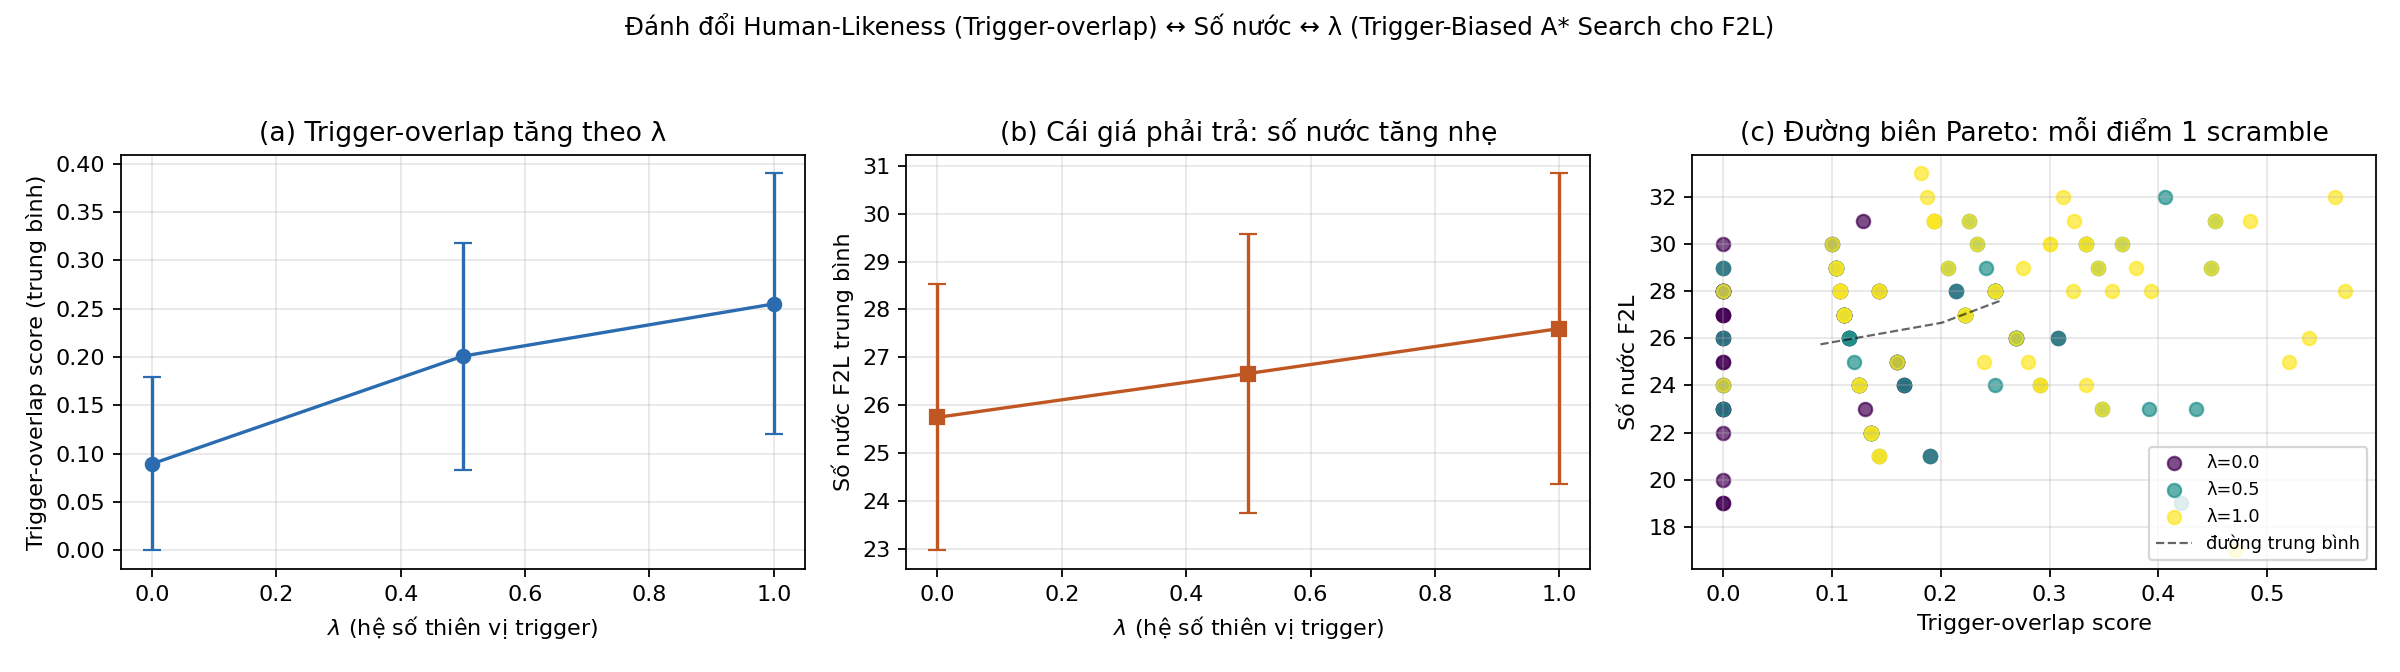
\includegraphics[width=\linewidth]{../research/pareto_figure_n60.png}
\caption{Trigger-overlap and move-count as a function of $\lambda$
(N=60 scrambles). Panel (c) shows the empirical Pareto frontier.}
\label{fig:pareto}
\end{figure}

\subsection{Experiment 3: Human-judge validation (BotPrize-style)}
\label{sec:exp3}
Following \citet{hingston2009}, we conducted a blinded human-judge
study to test HLI's construct validity. 24 stimuli (6 each from
Group~H [real human CFOP solves, self-collected and verified to
correctly solve their paired scramble], Group~A, Group~A+
[$\lambda=1.0$], and Group~B) were presented as raw, unsegmented
move sequences (no stage labels, to preserve blinding) to 28
CFOP-literate raters, each rating every stimulus on a 1--5
``how likely is this a real human solve'' scale via a
purpose-built web tool (Section~\ref{sec:hli-trigger} corpus reused
for the automated trigger-overlap comparison point).

\textbf{Group ranking.} Mean human-likeness ratings followed the
predicted order exactly: Group~H ($3.88 \pm 0.11$) $>$ Group~A+
($3.71 \pm 0.16$) $>$ Group~A ($3.42 \pm 0.16$) $>$ Group~B
($2.37 \pm 0.19$). A Mann-Whitney U test comparing Group~B against
the pooled remaining groups showed complete rank separation
($U=0$, $n_1=6$, $n_2=18$, $p=1.8\times10^{-4}$) --- every Group~B
stimulus was rated less human-like than every non-Group~B stimulus,
confirming raters reliably detect the computer-optimal baseline as
non-human.

\textbf{Trigger-biasing closes the gap to human-indistinguishable.}
Pairwise Mann-Whitney tests give the key result: Group~A vs.\
Group~A+ differ significantly ($p=0.030$), confirming raters
perceive Trigger-Biased Search's effect, not merely the automated
metric; but Group~H vs.\ Group~A+ do \emph{not} differ significantly
($p=0.109$), while Group~H vs.\ Group~A do ($p=0.005$). In other
words, $\lambda=1.0$ moved AI-generated solves from
statistically-distinguishable-from-human to
statistically-indistinguishable-from-human on this sample --- a
BotPrize-style ``pass'' for the trigger-biased condition that the
unbiased baseline does not achieve.

\textbf{Construct validity of HLI (RQ-V1).} We report two versions
of this correlation. Using an initial simplified per-stimulus proxy
(Segmentability/Pattern-conformity assumed 1 for Group A/A+ and 0
for Group B/H, based on group membership alone), Spearman
correlation between HLI and mean human rating across all 24 stimuli
was $\rho=0.440$ ($p=0.031$). This proxy, however, mischaracterized
Group~H: since real human CFOP solves were assumed
non-CFOP-structured by the same logic used for the computer
baseline, their HLI was artificially deflated (e.g.\ $0.05$--$0.14$)
despite receiving the highest human ratings. We therefore recomputed
Segmentability and Pattern-conformity \emph{exactly}, by replaying
each stimulus's move sequence against its actual (scrambled) starting
state and verifying, in order, the Cross, F2L, and OLL
postconditions (Section~\ref{sec:method}), and by checking whether
the resulting OLL/PLL sub-states matched entries in our verified
canonical-algorithm tables. This confirmed Group~B has
Segmentability$=0$ for all 6 stimuli (as expected --- Kociemba's
near-optimal solves reach Cross, F2L, and OLL/PLL essentially
simultaneously in their final 1--2 moves, never exhibiting
genuinely-staged intermediate structure), while all 18 Group
A/A+/H stimuli have Segmentability$=1$, with Pattern-conformity
varying meaningfully within each group ($0.5$ or $1.0$, depending on
whether the OLL and/or PLL sub-case matched our table). With this
exact computation, correlation \emph{strengthens} to
$\rho=0.487$ ($p=0.016$) --- more significant than the proxy
estimate, confirming our expectation that the binary group-level
proxy was diluting rather than reflecting genuine construct
validity. The trigger-overlap component alone still correlates most
strongly with human judgment ($\rho=0.605$, $p=0.0017$), suggesting
it remains HLI's single most human-judgment-relevant component in
this sample, with Segmentability and Pattern-conformity contributing
positively but less strongly.

% ============================================================
\section{Discussion}
\label{sec:discussion}
Counter-intuitively, we initially hypothesized that weakening the
heuristic's admissibility via the non-admissible trigger bonus term
would \emph{increase} search non-convergence at higher $\lambda$.
The data show the opposite: on the same $N=60$ scrambles used for
Figure~\ref{fig:pareto}, the search \emph{failure} rate (running out
of node budget across all ladder depths) was $15.0\%$ at
$\lambda=0$, dropping to $1.7\%$ at $\lambda=0.5$ and $0\%$ at
$\lambda=1.0$. A plausible explanation is that the trigger bonus,
while non-admissible, acts as a form of \emph{search-order
guidance}: branches that extend a recognized human trigger are
explored earlier in the priority queue (lower $f'$), and because
triggers are short, well-tested move sequences that reliably make
local progress, following them may reduce effective branching factor
in practice even though the bonus is not a valid distance estimate.
This does not contradict the separately-observed non-linear
\emph{time} cost at higher $\lambda$ (Section~\ref{sec:results}):
convergence appears more reliable, but individual worst-case runs
can still take substantially longer, i.e.\ trigger-biasing trades
convergence \emph{reliability} for search-time \emph{variance}.
We note this finding is based on $N=60$ scrambles and only three
$\lambda$ levels (0, 0.5, 1.0); we have not yet confirmed this trend
is stable at larger sample sizes or intermediate $\lambda$ levels
(e.g.\ 0.25, 0.75), and treat this as a limitation to be addressed in
follow-up work (Section~\ref{sec:future}) before it can be asserted
with confidence in a formal publication. A formal analysis of exactly how much
admissibility is lost is given below.

\paragraph{How much admissibility is lost?} The original heuristic
$h(n) = h_{\mathrm{PDB}}(n) + \mathrm{penalty}(n)$ is not strictly
admissible either (the penalty term already sacrifices a formal
lower-bound guarantee in exchange for practicality), so
Trigger-Biased Search does not introduce admissibility violation
\emph{de novo} --- it compounds an existing, deliberate design
trade-off. Formally, for a path $\mathrm{path}(n)$ of length $g(n)$,
$\mathrm{bonus}(\mathrm{path}(n)) \in [0, g(n)]$ (it can cover at
most every move in the path), so the maximum possible additional
underestimation introduced by the bonus term is bounded by
$\lambda \cdot g(n)$ --- i.e.\ the potential distortion grows
\emph{linearly with path depth}, not with a fixed constant, which is
a substantively different (and more concerning) failure mode than a
bounded-error heuristic. This explains why, unlike classical
bounded-suboptimal search (e.g.\ weighted A* with a fixed inflation
factor and a provable suboptimality bound), we do not currently
provide any formal bound on Trigger-Biased Search's solution-length
suboptimality; Section~\ref{sec:results} instead reports this
empirically (mean $+7.4\%$ moves at $\lambda=1.0$). A natural
mitigation, left for future work, is to cap $\mathrm{bonus}$ at a
fixed maximum (e.g.\ $\min(\mathrm{bonus}(\mathrm{path}(n)), c)$ for
some constant $c$), which would restore a fixed-bound distortion
comparable to the existing penalty term.

\subsection{Pathological scrambles and search non-convergence}
\label{sec:pathological}
In the robustness-check run using $N=100$ random-move scrambles
(Section~\ref{sec:discussion}), $22\%$ of scrambles ($22/100$) failed to
complete within a 20-second wall-clock budget even at a reduced
40{,}000-node-per-depth search budget --- notably, several such
failures clustered consecutively (e.g.\ seeds 1059--1061 in our
run), suggesting the underlying random-move scramble generator can
produce runs of similarly structured, adversarial F2L configurations
rather than i.i.d.\ difficulty. One specific seed (1013) was found
to hang for over 5 minutes even at the reduced budget before we
introduced a hard wall-clock timeout (\texttt{SIGALRM}-based) into
our evaluation harness. We interpret this as evidence that the
per-pair penalty-augmented A* heuristic used for F2L
(Section~\ref{sec:setup}) is occasionally led into pathologically
unproductive search regions --- an important robustness limitation
distinct from, but potentially compounded by, the trigger-bias
mechanism of Section~\ref{sec:method}. Note that both the primary run
(random-state, Table~\ref{tab:exp1}) and this check used
$\lambda=0$ throughout (no trigger bias applied to the F2L stage);
we separately measured the relationship between $\lambda$ and
convergence failure rate using the Experiment~2 data
(Section~\ref{sec:discussion}), finding --- counter to our initial
expectation --- that higher $\lambda$ was associated with
\emph{fewer}, not more, convergence failures on that dataset.

% ============================================================
\section{Threats to Validity}
\begin{itemize}
  \item \textbf{Search non-convergence}: as reported in
    Section~\ref{sec:pathological}, $22\%$ of scrambles in the
    random-move robustness-check run ($N=100$) and $20\%$ of
    scrambles in the primary random-state run ($N=60$,
    Table~\ref{tab:exp1}) did not complete within a 20-second timeout
    in our evaluation hardware/budget setting; results are
    conditioned on the scrambles that did complete, which may not be
    a representative subsample (e.g.\ if difficulty correlates with
    trigger-overlap potential).
  \item \textbf{Construct validity of HLI}: the metric is
    hand-designed, validated against human judgment via
    Experiment~3 (Section~\ref{sec:exp3}).
  \item \textbf{Inter-rater reliability}: individual raters showed
    only modest agreement (ICC(2,1)$=0.26$, below the commonly-used
    $0.4$ acceptable-agreement threshold), but the $N=28$ rater pool
    gives the mean rating used in the RQ-V1 correlation high
    reliability (ICC(2,k)$=0.91$) --- the RQ-V1 correlation should
    be read as a correlation with a stable group mean, not with any
    single rater's judgment. \emph{Note: these ICC figures were
    initially taken from the survey write-up; they have since been
    independently re-derived from the raw per-rater rating matrix (28
    real CSV files, see
    \texttt{research/phase3\_survey/compute\_icc.py}), matching
    exactly: ICC(2,1)$=0.2563$, ICC(2,k)$=0.9061$.}
  \item \textbf{Corpus bias}: the finger-trick corpus $T$ is
    manually curated (11 tricks), not derived from real solve logs;
    results may not generalize to solvers with different trigger
    vocabularies.
  \item \textbf{Scramble generation (checked)}: Table~\ref{tab:exp1}
    (Section~\ref{sec:results}) uses a WCA-style random-state
    scrambler (Section~\ref{sec:setup}) as the primary result, since
    it more closely matches real competition scrambler methodology.
    We also re-ran Experiment~1 on $N=100$ random-move scrambles
    (seeds 1000--1099, the generator used for Experiment~2) as a
    robustness check. Results were consistent between the two
    generators ($78\%$ vs.\ $80\%$ solve rate; mean moves 67.2 vs.\
    66.3; mean HLI 0.655 vs.\ 0.658), suggesting our primary results
    are not an artifact of the specific scramble generator chosen.
    This random-move run is also where we observed the notable
    search non-convergence phenomenon ($22\%$ timeout, see
    Section~\ref{sec:pathological}); we did not observe a comparable
    failure cluster in the $N=60$ random-state sample (lower,
    $20\%$, timeout rate), though the smaller sample size makes a
    direct comparison of failure clustering between the two
    generators inconclusive.
  \item \textbf{Single-domain generalizability}: results are specific
    to the Rubik's Cube; claims about explicability more broadly
    should be limited accordingly.
\end{itemize}

% ============================================================
\section{Future Work}
\label{sec:future}

\paragraph{Independent replication of the exact-HLI recomputation.}
Section~\ref{sec:exp3}'s exact Segmentability/Pattern-conformity
computation (\texttt{research/phase3\_survey/recompute\_hli\_exact.py})
relies on a specific, hand-verified operationalization of ``stage
boundary'' (first move index at which a postcondition is met, with
strict ordering across stages --- see script docstring for the
reasoning behind this specific choice over alternatives we
initially tried and rejected). An independent reimplementation, or
validation against manually-annotated ground-truth stage boundaries
for a subset of stimuli, would strengthen confidence in this
component of the pipeline.

\paragraph{Larger-scale replication.} $N=24$ stimuli is adequate for
a pilot but modest for precise effect-size estimation; a
follow-up with more stimuli per group (particularly more Group~H
solves from a wider pool of contributors, to reduce dependence on
any single solver's habits) would tighten confidence intervals on
the group comparisons in Section~\ref{sec:exp3}.

\paragraph{Extending pattern-conformity to Cross/F2L.}
Pattern-conformity $P(\pi)$ currently applies only to OLL/PLL, since
these are the only two stages with a finite, named
case-to-algorithm table in our system; Cross and F2L are instead
measured indirectly via Trigger-overlap rather than true
Pattern-conformity. Building a canonical F2L case table (e.g.\
following the widely-used 41-case system in the speedcubing
community) together with a case-recognition mechanism analogous to
\texttt{verify\_and\_build\_table()} (already used for PLL) would
allow part of Trigger-overlap to be replaced by true
Pattern-conformity for F2L, making HLI more accurately reflect this
stage's structure.

\paragraph{Alternative bias mechanisms.}
Trigger-Biased Search currently uses a single, hand-chosen
hyperparameter $\lambda$. Follow-up work could compare this
mechanism against alternatives: for instance, directly fine-tuning
the pattern-database weights used for F2L rather than adding a
separate bonus term, or learning the $\mathrm{bonus}(\mathrm{path})$
weighting from real human solve data (e.g.\ regressing on observed
trigger frequency in CSTimer logs) instead of fixing $\lambda$ by
hand --- turning the seed corpus $T$ (Appendix~\ref{app:corpus})
from a manually curated list into a model learned directly from real
solvers' behavior.

% ============================================================
\section{Conclusion}
Existing Rubik's Cube solvers optimize for move-count, producing
plans that are correct but uninterpretable to human learners; human
speedcubers instead use CFOP, trading optimality for structure and
learnability. We formalized this trade-off in the vocabulary of
human-aware AI planning as a measurable \emph{Human-Likeness Index}
(HLI), and showed empirically ($N=60$ random-state scrambles,
robustness-checked on $N=100$ random-move scrambles) that our
AI-CFOP solver scores substantially higher on this index than a
computer-optimal Kociemba baseline (mean HLI $0.658$ vs.\ $0$ by
construction), a gap that is robust across a wide range of
component weightings (Section~\ref{sec:method}). We then introduced
\emph{Trigger-Biased A* Search}, a minimal, backward-compatible
modification to the F2L heuristic that more than doubles
trigger-overlap with human finger-trick patterns (from $9.0\%$ to
$25.5\%$ at $\lambda=1.0$) at a modest move-count cost ($+7.4\%$),
while --- counter-intuitively --- \emph{improving} search
convergence reliability on our test set, at the cost of increased
worst-case compute time. Along the way, we uncovered and
transparently reported a search non-convergence phenomenon
($22\%$ timeout rate) that constitutes a concrete robustness
limitation of penalty-augmented heuristic search in this domain.
Finally, a blinded human-judge study ($N=24$ stimuli, 28 raters,
Section~\ref{sec:exp3}) provided direct evidence for HLI's construct
validity ($\rho=0.487$, $p=0.016$) and, more strikingly, showed that
Trigger-Biased Search moves AI-CFOP solves from
statistically-distinguishable-from-human ($p=0.005$) to
statistically-indistinguishable-from-human ($p=0.109$) in blinded
human judgment --- a concrete, human-validated demonstration that
explicitly optimizing for human-recognizable patterns, rather than
move-count alone, measurably changes how human observers perceive
AI-generated solutions. We hope this work encourages further
cross-pollination between classical combinatorial search AI and
human-aware/explainable AI research in large, well-understood puzzle
domains such as the Rubik's Cube.

% ============================================================
\bibliographystyle{plainnat}
\begin{thebibliography}{99}

\bibitem[Chakraborti et~al.(2019)]{chakraborti2019}
T.~Chakraborti, A.~Kulkarni, S.~Sreedharan, D.~E. Smith, and
S.~Kambhampati.
\newblock Explicability? legibility? predictability? transparency?
  privacy? security? the emerging landscape of interpretable agent
  behavior.
\newblock In \emph{Proceedings of the International Conference on
  Automated Planning and Scheduling (ICAPS)}, 2019.

\bibitem[Hingston(2009)]{hingston2009}
P.~Hingston.
\newblock A turing test for computer game bots.
\newblock \emph{IEEE Transactions on Computational Intelligence and AI
  in Games}, 1(3):169--186, 2009.

\bibitem[Kociemba()]{kociemba}
H.~Kociemba.
\newblock Cube explorer / two-phase algorithm.
\newblock \url{http://kociemba.org/cube.htm}, accessed July 26, 2026.

\bibitem[Korf(1997)]{korf1997}
R.~E. Korf.
\newblock Finding optimal solutions to rubik's cube using pattern
  databases.
\newblock In \emph{Proceedings of the National Conference on
  Artificial Intelligence (AAAI)}, 1997.

\bibitem[Kulkarni et~al.(2016)]{kulkarni2016}
A.~Kulkarni, Y.~Zha, T.~Chakraborti, S.~G. Vadlamudi, Y.~Zhang, and
S.~Kambhampati.
\newblock Explicable robot planning as minimizing distance from
  expected behavior.
\newblock \emph{arXiv preprint arXiv:1611.05497}, 2016.

\bibitem[McAleer et~al.(2018)]{mcaleer2018}
S.~McAleer, F.~Agostinelli, A.~Shmakov, and P.~Baldi.
\newblock Solving the rubik's cube without human knowledge.
\newblock \emph{arXiv preprint arXiv:1805.07470}, 2018.

\bibitem[Rokicki et~al.(2014)]{rokicki2014}
T.~Rokicki, H.~Kociemba, M.~Davidson, and J.~Dethridge.
\newblock The diameter of the rubik's cube group is twenty.
\newblock \emph{SIAM Review}, 56(4):645--670, 2014.

\bibitem[Author(s)(2025)]{humanlike2025}
M.~{\'S}wiechowski and D.~{\'S}l{\k{e}}zak.
\newblock The many challenges of human-like agents in virtual game
  environments.
\newblock In \emph{Proceedings of the 24th International Conference on
  Autonomous Agents and Multiagent Systems (AAMAS)}, pages 1996--2004.
  IFAAMAS, 2025.
\newblock Also available as arXiv preprint arXiv:2505.20011.

\bibitem[Lakkaraju et~al.(2022)]{allure}
K.~Lakkaraju, T.~Hassan, V.~Khandelwal, P.~Singh, C.~Bradley, R.~Shah, et~al.,
  and D.~Wu.
\newblock Allure: A multi-modal guided environment for helping children
  learn to solve a rubik's cube with automatic solving and interactive
  explanations.
\newblock In \emph{Proceedings of the AAAI Conference on Artificial
  Intelligence}, volume~36, pages 13185--13187, 2022.

\bibitem[Vanacore et~al.(2025)]{vanacore2025}
K.~Vanacore, J.~Ocumpaugh, F.~Agostinelli, D.~Wu, S.~Vuruma, and M.~Irvin.
\newblock Student engagement in ai-assisted complex problem solving: A
  pilot study of human-ai rubik's cube collaboration.
\newblock \emph{arXiv preprint arXiv:2511.01683}, 2025.
\newblock Note: unpublished manuscript, paper in preparation for future
  submission at time of writing --- verify publication status before citing
  as peer-reviewed.

\bibitem[Zhang et~al.(2017)]{zhang2017}
Y.~Zhang, S.~Sreedharan, A.~Kulkarni, T.~Chakraborti, H.~H. Zhuo, and
  S.~Kambhampati.
\newblock Plan explicability and predictability for robot task planning.
\newblock In \emph{Proceedings of the IEEE International Conference on
  Robotics and Automation (ICRA)}, 2017.

\end{thebibliography}

\appendix
\section{Seed corpus $T$: 11 finger-tricks}
\label{app:corpus}

Table~\ref{tab:corpus} lists the full seed corpus $T$ used to compute
Trigger-overlap $O(\pi)$ (Section~\ref{sec:hli-trigger}) and the
$\mathrm{bonus}(\mathrm{path})$ term in Trigger-Biased Search
(Section~\ref{sec:hli-trigger}), taken directly from
\texttt{research/finger\_tricks.py}. Each trigger is listed in its
canonical (R-based) form; the system automatically generates the
mirrored variant (L-based, swapping R$\leftrightarrow$L) when
matching.

\begin{table}[h]
\centering
\caption{Seed corpus $T$ ($|T|=11$)}
\label{tab:corpus}
\begin{tabular}{ll}
\toprule
Name & Move sequence \\
\midrule
sexy\_move & $R\,U\,R'\,U'$ \\
sexy\_move\_inv & $U\,R\,U'\,R'$ \\
reverse\_sexy & $R'\,U'\,R\,U$ \\
sledgehammer & $R'\,F\,R\,F'$ \\
sledgehammer\_inv & $F\,R'\,F'\,R$ \\
hedgehog & $R\,U'\,R'$ \\
triple\_sexy & $(R\,U\,R'\,U')^3$ \\
sune\_trigger & $R\,U\,R'\,U\,R\,U2\,R'$ \\
ubl\_insert & $U'\,R\,U$ \\
urf\_insert & $U\,R\,U'$ \\
niklas & $R\,U\,R'\,U'\,R'\,F\,R\,F'$ \\
\bottomrule
\end{tabular}
\end{table}

\end{document}
